\subsection{Forward proton analysis}
\begin{figure}[htbp]
  \centering
  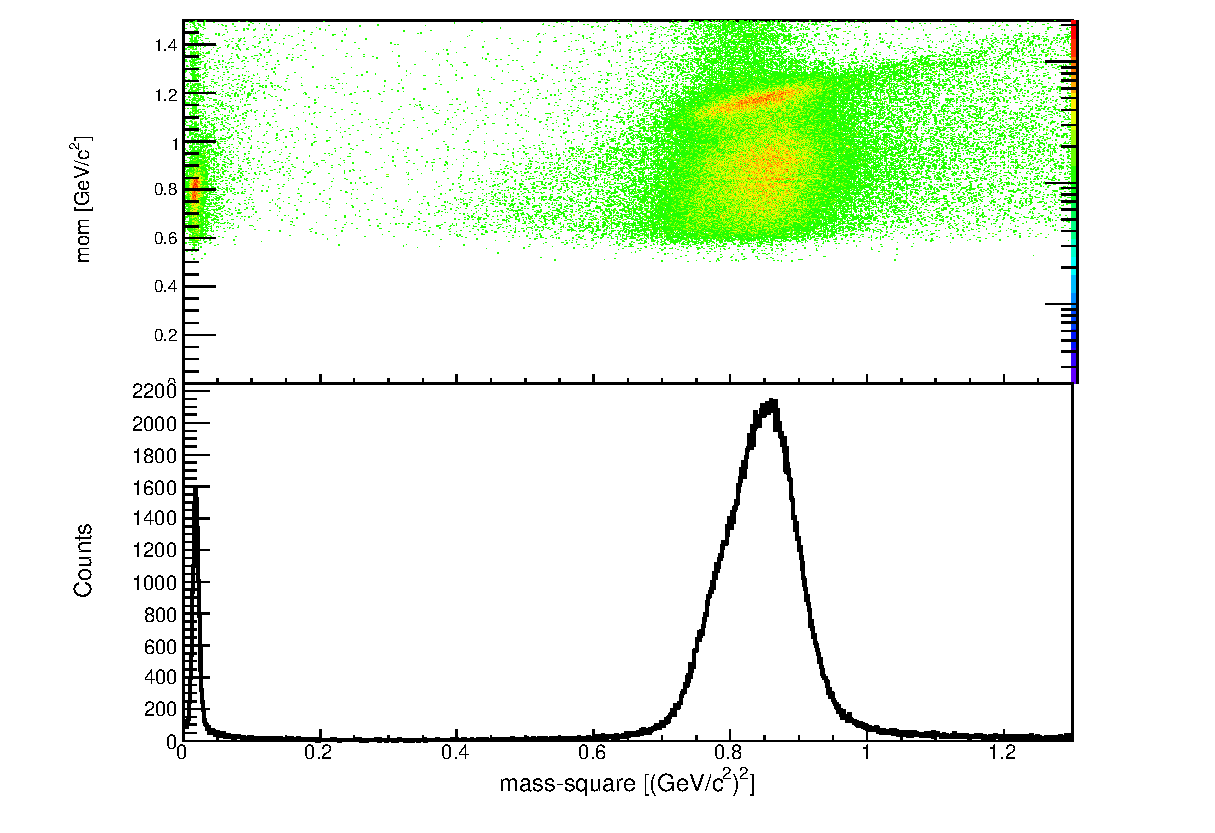
\includegraphics[width=10cm]{../pic/Dron/mass2_mom.eps}
  \caption{
    This figure shows scatterd plot mass-square and momentum of forward scattered positive charged particles and horizontal axis projection (down figure).
    The $\pi^+$ peak and the proton peak were seen around $m^2 \sim 0.02 [(GeV/c^2)^2]$ and $m^2 \sim 0.85 [(GeV/c^2)^2]$, respectively.
%    The $\pi^+$ peak is seen around $m^2 \sim 0.02 [(GeV/c^2)^2]$ and the proton peak is seen around $m^2 \sim 0.9 [(GeV/c^2)^2]$
  }
  \label{fig:FC_mass2_mom}
\end{figure}

Forward proton was bended by the Ushiwaka magnet and fired the PC/CVC,
so the fight length of forward charged particle was depend on the momentum and scattered angle.
The flight length was evaluated from the reaction vertex point, position at just upstream of the Ushiwaka magnet measured by the FDC and counter hit position.
The trajectory was calculated by the third order Rungge-Kutta method with magnetic field map.
The field map was calculated by the Opera which is finite element method software\cite{Opera} and absolute value was scaled by measured value.
The velocity ($\beta$) was calculated using the TOF method.
The momentum was estimated from the bending angle and mass-square was reconstructed from the velocity and momentum which is same method of decayed particle detected by the CDS.
Fig.\ref{fig:FC_mass2_mom} shows scatter plot of mass-square and momentum.
Events whose $m^{2}>0.5 [(GeV/c^2)^2]$ are accepted as the proton. Fig.\ref{fig:KP_MM} shows the $d(K^-, p)$ missing mass.

\begin{figure}[htbp]
  \centering
  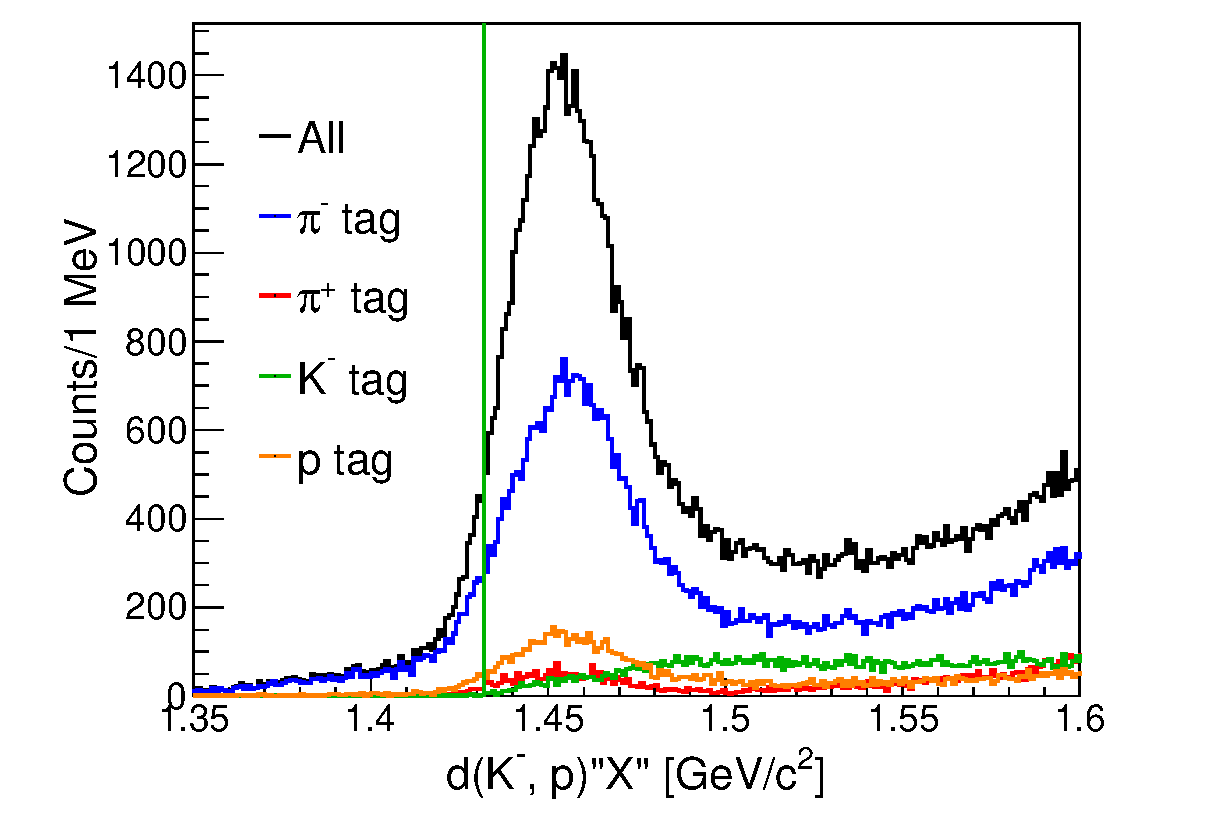
\includegraphics[width=10cm]{../pic/Run68/KP_ana/KP_MM.eps}
  \caption{
    %% todo 推敲する
    This figure shows $d(K^-, p)"X"$ missing mass spectra.
    Black plot indicates whole data and color plots indicates CDS particles tagged data.
    These plots was adopted time offset calibration using well known particles identified by the missing mass which is described at Sec\ref{sec:KP_timeoffset}.
  }
  \label{fig:KP_MM}
\end{figure}

The momentum was measured by the TOF method, althought flight length was function of the scattered angle and the momentum.
The position just above the Ushiwaka magnent was masured by the FDC1 and the trajectory was exploarted to the fired counter.
The trajectory of the forward scattered charged particle was calculated by the theird order Rungge-Kutta method using the magnetic field calculated by the Opera\cite{Opera}.




